\vspace{2mm}
\begin{figure}[h!]

\tikzset{every picture/.style={line width=0.75pt}} %set default line width to 0.75pt        

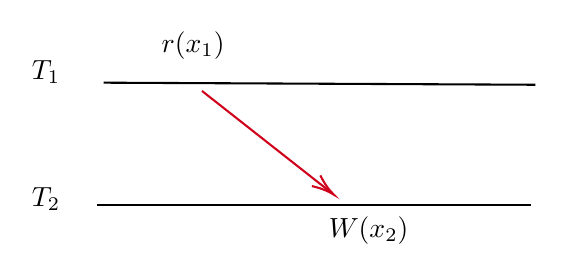
\begin{tikzpicture}[x=0.75pt,y=0.75pt,yscale=-1,xscale=1]
%uncomment if require: \path (0,300); %set diagram left start at 0, and has height of 300

%Straight Lines [id:da9500410641573396] 
\draw    (50.56,42) -- (258.56,43) ;
%Straight Lines [id:da7796185686481738] 
\draw    (47.56,101) -- (256.56,101) ;
%Straight Lines [id:da9563274467788809] 
\draw [color={rgb, 255:red, 208; green, 2; blue, 27 }  ,draw opacity=1 ]   (98,46) -- (159.99,94.76) ;
\draw [shift={(161.56,96)}, rotate = 218.19] [color={rgb, 255:red, 208; green, 2; blue, 27 }  ,draw opacity=1 ][line width=0.75]    (10.93,-3.29) .. controls (6.95,-1.4) and (3.31,-0.3) .. (0,0) .. controls (3.31,0.3) and (6.95,1.4) .. (10.93,3.29)   ;

% Text Node
\draw (14.5,30) node [anchor=north west][inner sep=0.75pt]   [align=left] {$T_1$};
% Text Node
\draw (14.5,91) node [anchor=north west][inner sep=0.75pt]   [align=left] {$T_2$};
% Text Node
\draw (157.56,105) node [anchor=north west][inner sep=0.75pt]   [align=left] {$W(x_2)$};
% Text Node
\draw (77,16) node [anchor=north west][inner sep=0.75pt]   [align=left] {$r(x_1)$};


\end{tikzpicture}
    \caption{Anti-dependency between the read of $T_1$ and the write of $T_2$}
\end{figure}
\vspace{2mm}